\subsubsection{\textit{Câu 1}}

\noindent\textbf{\large Đề bài:} Viết chương trình hợp ngữ Assembly cho phép nhập vào một số và in ra màn hình giai thừa của số đó.

\vspace{0.5cm}
\noindent\textbf{\large Biểu diễn bằng Flowchart:} hình \ref{fig:flowchart-1}

\begin{figure}[H]
    \centering
    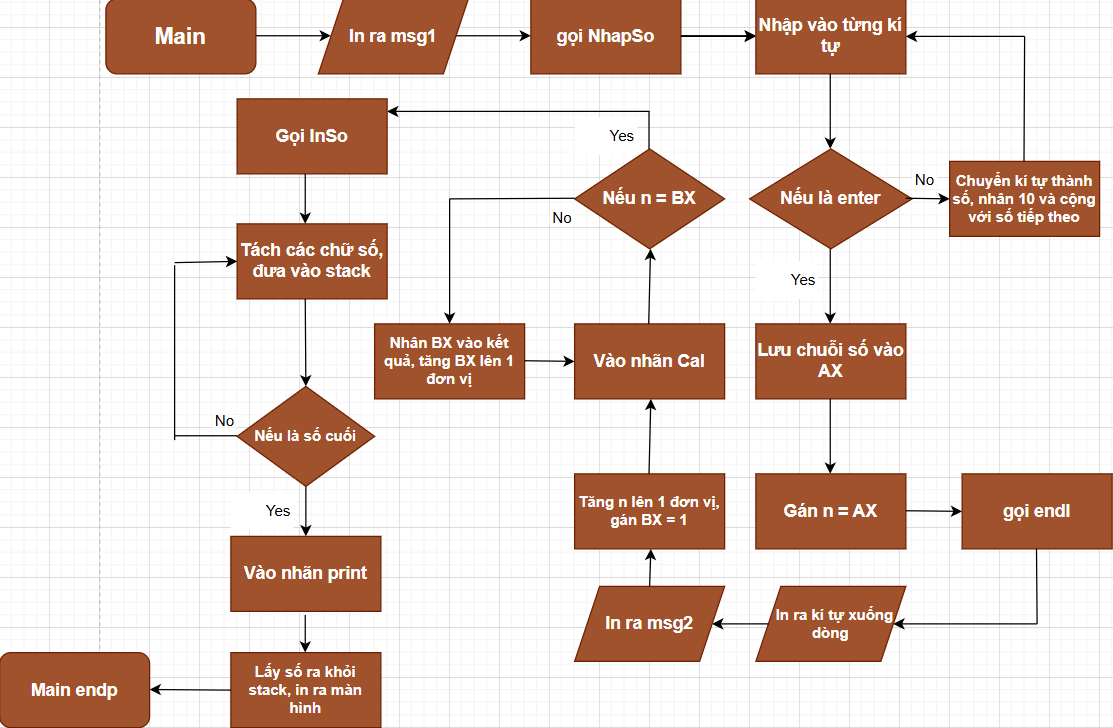
\includegraphics[width=1\textwidth]{Images/Flowchart/Flowchart-1.png}
    \caption{Flowchart tính giai thừa 1 số}
    \label{fig:flowchart-1}
\end{figure}

\vspace{0.5cm}
\noindent\textbf{\large Mã nguồn assembly 8086:}
\begin{lstlisting}[style=asm, caption={Mã nguồn câu 1}]
    .model small               ;Khoi tao che do bo nho la small
    .stack 100                 ;Khoi tao kich thuoc ngan xep
    .data                      ;Khoi tao cac bien
        crlf db 13, 10, '$'      
        x dw ?
        y dw ? 
        n dw ? 
        msg1 db 'Nhap vao 1 so: $'
        msg2 db 'Giai thua cua so da nhap la: $'
    .code
    main proc                  ;Ham chinh cua chuong trinh
        mov ax, @data
        mov ds, ax             ;Khoi tao thanh ghi ds
        
        mov ah, 9              ;In ra msg1
        lea dx, msg1
        int 21h
        
        call NhapSo            ;Thuc hien nhap so
        mov n, ax              ;Luu so vua nhap vao n
        call endl              ;Xuong dong
        
        mov ah, 9              ;In ra msg2
        lea dx, msg2
        int 21h
        
        inc n                  ;Tang n len 1 don vi
        mov bx, 1              ;Khoi tao thanh ghi bx
        mov ax, 1              ;Khoi tao thanh ghi ax de luu ket qua
        Cal:
            cmp bx, n          ;So sanh bx voi n
            je break           ;Neu bx = n thi thuc hien break
            mul bx             ;Neu bx != n thi nhan ax voi bx, luu vao ax
            inc bx             ;Tang bx len 1 don vi
            jmp Cal            ;Tiep tuc lap de tinh giai thua
        break:
        call InSo              ;In ra ket qua
        
        mov ah, 4ch            ;Ket thuc chuong trinh
        int 21h
    main endp 
    
    NhapSo proc                ;Ham con de nhap so
        mov x, 0               ;Khoi tao x = 0
        mov y, 0               ;Khoi tao y = 0
        mov bx, 10             ;Khoi tao bx = 10
        nhap:   
            mov ah, 1          ;Nhap 1 ki tu
            int 21h 
            cmp al, 13         ;Neu ki tu la dau enter thi chay vao nhapxong
            je nhapxong
            sub al, '0'        ;Neu ki tu khong phai enter thi bien doi thanh so
            mov ah, 0
            mov y, ax          ;Luu so vua nhap vao y
            mov ax, x
            mul bx             ;Lay ax * bx, ket qua luu vao ax
            add ax, y          ;Lay ax + y, ket qua luu vao ax
            mov x, ax          
            jmp nhap           ;Tiep tuc lap den khi nhap xong
        nhapxong:
            mov ax, x          ;Luu so da nhap vao thanh ghi ax
        ret
    NhapSo endp 
    
    endl proc                   ;Ham con de xuong dong
        push ax
        push dx
        
        mov ah, 9               ;In ra ki tu xuong dong
        lea dx, crlf
        int 21h
        
        pop dx
        pop ax
        ret
    endl endp  
    
    InSo proc                  ;Ham con de in so
        push ax
        push bx
        push cx
        push dx
        
        mov bx, 10             ;Khoi tao bx = 10
        mov cx, 0              ;Khoi tao cx = 0
        beforePrint:
            mov dx, 0
            div bx             ;Thuc hien ax / bx, phan nguyen luu vao ax, phan du luu vao dx
            push dx            ;Day phan du vao ngan xep
            inc cx             ;Tang cx 
            cmp ax, 0          ;Neu ax > 0 thi tiep tuc tach so
            jg beforePrint
        print:
            pop dx             ;Lap phan du ra khoi ngan xep
            mov ah, 2          
            add dx, '0'        ;Bien doi so thanh ki tu
            int 21h            ;In ra man hinh
            loop print         ;Lap cho den khi in xong
        
        pop dx
        pop cx
        pop bx
        pop ax
        ret
    InSo endp
    
    end main
\end{lstlisting}

\vspace{0.5cm}
\noindent\textbf{\large Giao diện hiển thị: } hình \ref{fig:result-1}

\begin{figure}[H]
    \centering
    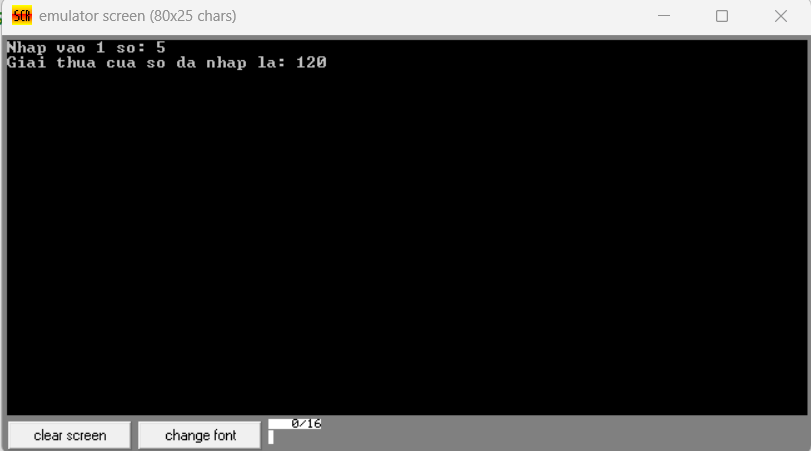
\includegraphics[width=0.8\textwidth]{Images/Result/B1.png}
    \caption{Giao diện hiển thị câu 1}
    \label{fig:result-1}
\end{figure}